% questions.tex —— 2017 年·北京卷·文科 · 题目内容片段（无答案）
% 由 tools/generate_projects.py 依来源总账自 2017/2017_数学真题_北京文_试题.md 生成，勿手改（改源 MD 后重跑）

\gkpart{数学}

\begin{gktip}
\textbf{来源说明}：本题面依据固定源 PDF 两页 A3 页面逐题核对，原卷印刷页码 1033–1034。固定源不附答案；本文件仅为题面规范源。
\end{gktip}

\gkpart{一、选择题}

\begin{question}
\gkti{1}
已知全集 $U=\mathbb R$，集合 $A=\{x\mid x<-2\text{ \text{或} }x>2\}$，则 $\complement_U A=$（　）

\begin{itemize}
\item (A) $(-2,2)$
\item (B) $(-\infty,-2)\cup(2,+\infty)$
\item (C) $[-2,2]$
\item (D) $(-\infty,-2]\cup[2,+\infty)$
\end{itemize}

\end{question}
\begin{question}
\gkti{2}
若复数 $(1-i)(a+i)$ 在复平面内对应的点在第二象限，则实数 $a$ 的取值范围是（　）

\begin{itemize}
\item (A) $(-\infty,1)$
\item (B) $(-\infty,-1)$
\item (C) $(1,+\infty)$
\item (D) $(-1,+\infty)$
\end{itemize}

\Needspace{0.4\textheight}
\end{question}
\begin{question}
\gkti{3}
执行如图所示的程序框图，输出的 $S$ 值为（　）
\nopagebreak[4]
\begin{center}\begin{tikzpicture}[>=stealth,thick,
  node distance=8mm,
  term/.style={draw,rounded corners=3pt,minimum width=22mm,minimum height=7mm},
  proc/.style={draw,minimum width=30mm,minimum height=8mm,align=center},
  test/.style={draw,diamond,aspect=2.2,inner sep=1pt,align=center},
  io/.style={draw,trapezium,trapezium left angle=70,trapezium right angle=110,
    minimum width=27mm,minimum height=8mm,align=center}]
  \node[term] (start) at (-2,0) {开始};
  \node[proc] (init) at (-2,-1.15) {$k=0,\ s=1$};
  \node[test] (test) at (0,-2.65) {$k<3$？};
  \node[proc] (inc) at (3,-2.65) {$k=k+1$};
  \node[proc] (update) at (3,-1.15) {$s=\dfrac{s+1}{s}$};
  \node[io] (out) at (0,-4.15) {输出 $s$};
  \node[term] (stop) at (0,-5.25) {结束};
  \draw[->] (start)--(init);
  \draw[->] (init)--(test);
  \draw[->] (test.east)--node[above]{是}(inc.west);
  \draw[->] (inc.north)--(update.south);
  \draw[->] (update.west)--++(-1.05,0)|-(test.north);
  \draw[->] (test.south)--node[right]{否}(out.north);
  \draw[->] (out)--(stop);
\end{tikzpicture}
\end{center}
\nopagebreak[4]
\begin{itemize}
\item (A) $2$
\item (B) $\dfrac32$
\item (C) $\dfrac53$
\item (D) $\dfrac85$
\end{itemize}

\end{question}
\begin{question}
\gkti{4}
\Needspace{5\baselineskip}
若 $x,y$ 满足

\nopagebreak[4]
\[
\begin{cases}
x\leqslant3,\\
x+y\geqslant2,\\
y\leqslant x,
\end{cases}
\]

则 $x+2y$ 的最大值为（　）

\begin{itemize}
\item (A) $1$
\item (B) $3$
\item (C) $5$
\item (D) $9$
\end{itemize}

\end{question}
\begin{question}
\gkti{5}
已知函数 $f(x)=3^x-\left(\dfrac13\right)^x$，则 $f(x)$（　）

\begin{itemize}
\item (A) 是偶函数，且在 $\mathbb R$ 上是增函数
\item (B) 是奇函数，且在 $\mathbb R$ 上是增函数
\item (C) 是偶函数，且在 $\mathbb R$ 上是减函数
\item (D) 是奇函数，且在 $\mathbb R$ 上是减函数
\end{itemize}

\Needspace{0.4\textheight}
\end{question}
\begin{question}
\gkti{6}
某三棱锥的三视图如图所示，则该三棱锥的体积为（　）
\nopagebreak[4]
\begin{center}\begin{tikzpicture}[thick,>=stealth,line cap=round,line join=round,
  dim/.style={<->,thin}, every node/.style={font=\small}]
  % Front view: right triangular face, with the source dimensions 4 and 5.
  \draw (0,0)--(0,2.4)--(3,0)--cycle;
  \draw[dim] (-.42,0)--(-.42,2.4) node[midway,left]{4};
  \draw[thin] (-.12,0)--(-.52,0) (-.12,2.4)--(-.52,2.4);
  \draw[dim] (0,-.42)--(3,-.42) node[midway,below]{5};
  \draw[thin] (0,-.12)--(0,-.52) (3,-.12)--(3,-.52);
  \node at (1.5,2.85) {正（主）视图};
  % Side view: triangular elevation, width 3.
  \draw (5,0)--(7.4,2.4)--(7.4,0)--cycle;
  \draw[dim] (5,-.42)--(7.4,-.42) node[midway,below]{3};
  \draw[thin] (5,-.12)--(5,-.52) (7.4,-.12)--(7.4,-.52);
  \node at (6.2,2.85) {侧（左）视图};
  % Plan: rectangular footprint and the two crossing diagonals, one hidden.
  \draw (0,-3.15) rectangle (3,-4.35);
  \draw (0,-3.15)--(3,-4.35);
  \draw[dashed] (0,-4.35)--(3,-3.15);
  \node at (1.5,-4.8) {俯视图};
\end{tikzpicture}
\end{center}
\nopagebreak[4]
\begin{itemize}
\item (A) $60$
\item (B) $30$
\item (C) $20$
\item (D) $10$
\end{itemize}

\end{question}
\begin{question}
\gkti{7}
设 $\boldsymbol m,\boldsymbol n$ 为非零向量，则“存在负数 $\lambda$，使得 $\boldsymbol m=\lambda\boldsymbol n$”是“$\boldsymbol m\cdot\boldsymbol n<0$”的（　）

\begin{itemize}
\item (A) 充分而不必要条件
\item (B) 必要而不充分条件
\item (C) 充分必要条件
\item (D) 既不充分也不必要条件
\end{itemize}

\end{question}
\begin{question}
\gkti{8}
根据有关资料，围棋状态空间复杂度的上限 $M$ 约为 $3^{361}$，而可观测宇宙中普通物质的原子总数 $N$ 约为 $10^{80}$，则下列各数中与 $\dfrac MN$ 最接近的是（　）

（参考数据：$\lg3\approx0.48$）

\begin{itemize}
\item (A) $10^{33}$
\item (B) $10^{53}$
\item (C) $10^{73}$
\item (D) $10^{93}$
\end{itemize}

\end{question}
\gkpart{二、填空题}

\begin{question}
\gkti{9}
在平面直角坐标系 $xOy$ 中，角 $\alpha$ 与角 $\beta$ 均以 $Ox$ 为始边，它们的终边关于 $y$ 轴对称，若 $\sin\alpha=\dfrac13$，则 $\sin\beta=$ \gkblank{}。

\end{question}
\begin{question}
\gkti{10}
若双曲线 $x^2-\dfrac{y^2}{m}=1$ 的离心率为 $\sqrt3$，则实数 $m=$ \gkblank{}。

\end{question}
\begin{question}
\gkti{11}
已知 $x\geqslant0,\ y\geqslant0$，且 $x+y=1$，则 $x^2+y^2$ 的取值范围是 \gkblank{}。

\end{question}
\begin{question}
\gkti{12}
已知点 $P$ 在圆 $x^2+y^2=1$ 上，点 $A$ 的坐标为 $(-2,0)$，$O$ 为原点，则 $\overrightarrow{AO}\cdot\overrightarrow{AP}$ 的最大值为 \gkblank{}。

\end{question}
\begin{question}
\gkti{13}
能够说明“设 $a,b,c$ 是任意实数。若 $a>b>c$，则 $a+b>c$”是假命题的一组整数 $a,b,c$ 的值依次为 \gkblank{}。

\end{question}
\begin{question}
\gkti{14}
某学习小组由学生和教师组成，人员构成同时满足以下三个条件：

① 男学生人数多于女学生人数；

② 女学生人数多于教师人数；

③ 教师人数的两倍多于男学生人数。

(1)   若教师人数为 $4$，则女学生人数的最大值为 \gkblank{}；

(2)   该小组人数的最小值为 \gkblank{}。

\end{question}
\gkpart{三、解答题}

\begin{question}
\gkti{15}
已知等差数列 $\{a_n\}$ 和等比数列 $\{b_n\}$ 满足 $a_1=b_1=1$，$a_2+a_4=10$，$b_2b_4=a_5$。

(1)   求 $\{a_n\}$ 的通项公式；

(2)   求和：$b_1+b_3+b_5+\cdots+b_{2n-1}$。

\end{question}
\begin{question}
\gkti{16}
已知函数 $f(x)=\sqrt3\cos\left(2x-\dfrac\pi3\right)-2\sin x\cos x$。

(1)   求 $f(x)$ 的最小正周期；

(2)   求证：当 $x\in\left[-\dfrac\pi4,\dfrac\pi4\right]$ 时，$f(x)\geqslant-\dfrac12$。

\Needspace{0.4\textheight}
\end{question}
\begin{question}
\gkti{17}
某大学艺术专业 $400$ 名学生参加某次测评，根据男女学生人数比例，使用分层抽样的方法从中随机抽取了 $100$ 名学生，记录他们的分数，将数据分成 $7$ 组：$[20,30),\allowbreak[30,40),\allowbreak\cdots,\allowbreak[80,90]$，并整理得到如下频率分布直方图：
\nopagebreak[4]
\begin{center}\begin{tikzpicture}[x=.45cm,y=1.05cm,thick,>=stealth,
  every node/.style={font=\small}]
  % The first three heights are read from the drawn geometry relative to the
  % labelled 0.01 grid (about 0.002, 0.003, 0.005); those values are not printed
  % labels in the source and are represented only by unlabelled bar heights.
  \draw[->] (0,0)--(10,0) node[right]{分数};
  \draw[->] (0,0)--(0,4.8) node[above]{$\dfrac{\text{频率}}{\text{组距}}$};
  \foreach \x/\lab in {0/0,2/20,3/30,4/40,5/50,6/60,7/70,8/80,9/90}
    \node[below=2pt] at (\x,0) {\lab};
  \draw[dashed,thin] (0,1)--(5,1);
  \draw[dashed,thin] (0,2)--(6,2);
  \draw[dashed,thin] (0,4)--(7,4);
  \node[left=2pt] at (0,1) {$0.01$};
  \node[left=2pt] at (0,2) {$0.02$};
  \node[left=2pt] at (0,4) {$0.04$};
  \draw (2,0) rectangle (3,.2);
  \draw (3,0) rectangle (4,.3);
  \draw (4,0) rectangle (5,.5);
  \draw (5,0) rectangle (6,1);
  \draw (6,0) rectangle (7,2);
  \draw (7,0) rectangle (8,4);
  \draw (8,0) rectangle (9,2);
  \draw[dashed,thin] (6,2)--(6.7,2);
\end{tikzpicture}
\end{center}
\nopagebreak[4]
(1)   从总体的 $400$ 名学生中随机抽取一人，估计其分数小于 $70$ 的概率；

(2)   已知样本中分数小于 $40$ 的学生有 $5$ 人，试估计总体中分数在区间 $[40,50)$ 内的人数；

(3)   已知样本中有一半男生的分数不小于 $70$，且样本中分数不小于 $70$ 的男女生人数相等。试估计总体中男生和女生人数的比例。

\Needspace{0.4\textheight}
\end{question}
\begin{question}
\gkti{18}
如图，在三棱锥 $P-ABC$ 中，$PA\perp AB$，$PA\perp BC$，$AB\perp BC$，$PA=AB=BC=2$，$D$ 为线段 $AC$ 的中点，$E$ 为线段 $PC$ 上一点。

(1)   求证：$PA\perp BD$；

(2)   求证：平面 $BDE\perp$ 平面 $PAC$；

(3)   当 $PA\parallel$ 平面 $BDE$ 时，求三棱锥 $E-BCD$ 的体积。
\nopagebreak[4]
\begin{center}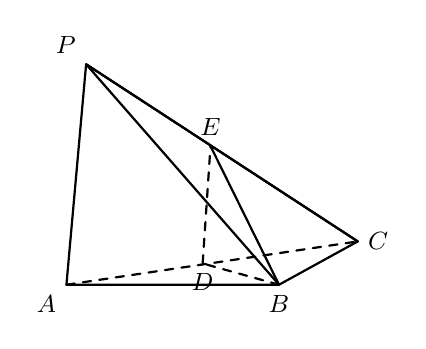
\begin{tikzpicture}[thick,line cap=round,line join=round,
  every node/.style={font=\small}]
  \coordinate (P) at (0,2.8);
  \coordinate (A) at (-.25,0);
  \coordinate (B) at (2.45,0);
  \coordinate (C) at (3.45,.55);
  \coordinate (D) at (1.48,.27);
  \coordinate (E) at (1.58,1.76);
  \draw (P)--(A)--(B)--(C)--(P)--(B);
  \draw (P)--(C);
  \draw[dashed] (A)--(C);
  \draw (B)--(E);
  \draw[dashed] (D)--(E) (B)--(D);
  \node[above left] at (P) {$P$};
  \node[below left] at (A) {$A$};
  \node[below] at (B) {$B$};
  \node[right] at (C) {$C$};
  \node[below] at (D) {$D$};
  \node[above] at (E) {$E$};
\end{tikzpicture}
\end{center}
\nopagebreak[4]
\end{question}
\begin{question}
\gkti{19}
已知椭圆 $C$ 的两个顶点分别为 $A(-2,0),\ B(2,0)$，焦点在 $x$ 轴上，离心率为 $\dfrac{\sqrt3}{2}$。

(1)   求椭圆 $C$ 的方程；

(2)   点 $D$ 为 $x$ 轴上一点，过 $D$ 作 $x$ 轴的垂线交椭圆 $C$ 于不同的两点 $M,N$，过 $D$ 作 $AM$ 的垂线交 $BN$ 于点 $E$。求证：$\triangle BDE$ 与 $\triangle BDN$ 的面积之比为 $4:5$。

\end{question}
\begin{question}
\gkti{20}
已知函数 $f(x)=e^x\cos x-x$。

(1)   求曲线 $y=f(x)$ 在点 $(0,f(0))$ 处的切线方程；

(2)   求函数 $f(x)$ 在区间 $\left[0,\dfrac\pi2\right]$ 上的最大值和最小值。

\end{question}